
%%%%%%%%%%%%%%%%%%%%%%%%%%%%%%%%%%%%%%%%%%%%%%%%%%%%%%%%%%%%%%%%%%%%%%%%
%Para las ecuaciones siempre es Ec.(n).
%Para las figuras siempre es Fig.n, incluso en el caption de la figura. Tambien las Tablas
%Para las referencias es [n]
%%%%%%%%%%%%%%%%%%%%%%%%%%%%%%%%%%%%%%%%%%%%%%%%%%%%%%%%%%%%%%%%%%%%%%%%

\documentclass[
reprint,
%notitlepage,
%superscriptaddress,
%groupedaddress,
%unsortedaddress,
%runinaddress,
%frontmatterverbose, 
%preprint,
%showpacs,preprintnumbers,
%nofootinbib,
%nobibnotes,
%bibnotes,
%11 pt,
amsmath,
amssymb,
aps,
pra,
%prb,
%rmp,
%tightenlines %esto hizo el milagro de sacar los espacios en blancos estocásticos (?)
 %prstab,
%prstper,
%floatfix,\textbf{}
]{revtex4-1} %Instalar primero para usarlo. Paquete malo.

%\documentclass[onecolumn, aps, amsmath,amssymb ]{article}
\usepackage{lipsum}  
\usepackage{graphicx}% Include figure files
\usepackage{subfig}
\usepackage{braket}
\usepackage{comment} %comment large chunks of text
\usepackage{dcolumn}% Align table columns on decimal point
\usepackage{bm}% bold math
%\usepackage{hyperref}% add hypertext capabilities
\usepackage[mathlines]{lineno}% Enable numbering of text and display math
%\linenumbers\relax % Commence numbering lines
\usepackage{mathtools} %% Para el supraíndice

\usepackage[nice]{nicefrac}

%%%%%%%El Señor Español%%%%%%%%%%%%%%%%%%%%%%%%%%%
\usepackage[utf8]{inputenc} %acento
\usepackage[
spanish, %El lenguaje.
es-tabla, %La tabla y no cuadro.
activeacute, %El acento.
es-nodecimaldot %Punto y no coma con separador de números
]{babel}
\usepackage{microtype} %para hacerlo más bonito :33 como vos (?) 
%%%%%%%%%%%%%%%%%%%%%%%%%%%%%%%%%%%%%%%%%%%%%%%%%%%
%%%%%%%%% Para que las imágenes se queden dónde las quiero (?
\usepackage{float}
%%%%%%%%%%

%%%%%%%%Cambia a Fig de Figure%%%%%%%%%%
\makeatletter
\renewcommand{\fnum@figure}{Fig. \thefigure} 
\makeatother
%%%%%%%%%%%%%%%%%%%%%%%%%%%%%%%%%%%%%%%%
\raggedbottom


\begin{document}
%%%%%%%%%%%%%%%%%%%%%%%%%%%%%%%%%%Título%%%%%%%%%%%%%%%%%%%%%%%%%%%%%%%%%%%%%%
%%%%%%%%%%%%%%%%%%%%%%%%%%%%%%%%%%%%%%%%%%%%%%%%%%%%%%%%%%%%%%%%%%%%%%%%%%%%%%

\title{Clases  de Redes neuronales}
\author{Evelyn~G.~Coronel}

\affiliation{
Redes Neuronales - Instituto Balseiro\\}

\date[]{\lowercase{\today}} %%lw para lw, [] sin date

\begin{abstract}

\end{abstract} 
\maketitle
%%%%%%%%%%%%%%%%%%%%%%%%%%%%%%%%%%%%%%%%%%%%%%%%%%%%%%%%%%%%%%%%%%%%%%%%%%%%%%%%%%%
% Podemos usar cualquiera de los dos comandos: \input o \include para incluir el texto
%\input{./Capitulo1/cap1.tex}


\section{Clase del 12/02/2020}


\subsection{Redes Neuronales}

\subsubsection{Propiedades electricas de las neuronas}

\begin{itemize}
	\item Líquidos Celulares
		\begin{itemize}
			\item Controla la resistividad de la neurona
			\item La resistividad es $\approx 1 \Omega m$. Dió el ejemplo de un volumen de líquido como  una caja o como una esfera, ya que la resistencia del volumen va como $\nicefrac{Area}{Volumen}$
			\end{itemize}
	\item Membrana Celular
		\begin{itemize}
			\item Tiene una resistencia característica de $\approx 1 M\Omega mm^2$. 
			\item Esta membrana dificulta la entrada de corriente al interior de la neurona. 
			\item Capacitancia de $\approx 10 nF/mm^2$. Meramente geometrica
			\item Es como un circuito RC de tiempo de respuesta de 10 ms, esto limita el rango de tiempo en el que puedo estudiar la neurona desde afuera.
			\item La resistividad es dinamica, depende de la actividad , las proteinas etc
			\item La membrana tiene una estructura de bicapa fosfobarica, además de proteínas de canas, que filtran distitnos minerales. También se encuentran las proteínas bomba, que se encargan de ingresar otros minerales dentro de la neurona.
			\item El canal puede tener variaciones y dejar pasar o no dentro de la celula.
		\end{itemize}
\end{itemize}

Gráfico de la membrana

Gráfico de la corriente en función del tiempo


\subsection{Modelo simplificado de la membrana}
Dibujito
\begin{enumerate}
	\item La membrana se encuentra sumergida en agua, al agregar sal (común por ejemplo), esta sal se ioniza
	\item Tenemos canales de K, es decir, filtros que dejan pasar el K
	\item Por eso tengo concentración de K en ambos lados de la membrana
	\item Para llegar al equilibrio, juegan un papel 
	\begin{itemize}
		\item Fuerza difusiva 
		\item- la fuerza electrostática
	\end{itemize}
	\item Tengo una diferencia de potencial proque iones, y esto es una diferencia de energía porque $E = Vq$
	\item La probabilidad de que ingrese mas K adentro es de Boltzmann porque es así, (ecuación de Nersrnt?)
	\begin{equation}
		e^{-\Delta E / KT} = \frac{[K]_out}{K_in}
	\end{equation}
	\item Despejando la ec anterior, tenemos que
	\begin{equation}
		V = \frac{KT}{e} ln(\frac{[A]_out}{A_in})
	\end{equation}
	de para temperatura ambiente $\frac{KT}{e} = 60 mV$. EL potencial se ve afectado principalmente por la temperatura del huesped.
\end{enumerate}

\subsection{Neurona Real}
\begin{table}
\centering
\begin{tabular}{c|c|c|c}
Cosas & In & Out & V \\
Na+ & 5-15 mM & 145 & + \\
K+  & 140  &  5  & - \\
Cl- & 4 	& 140 & +\\
Ca+ & 0.1 $\mu$M& 2.5 - 5 & +\\ 
\end{tabular}
\end{table}

Siempre Sale K y entra Na

\subsection{Teoría de Transporte Goldman-Hudgkin-Katz}

dibujito potencial

De [A](z)

Las corrientes de:
\begin{itemize}
	\item Difusion 
\begin{equation}
	j_a^D= - D_A \frac{d[A]}{dz}
\end{equation}
	\item Electrostatico
\begin{equation}
	j_A^e = \mu_A \frac{q_A V}{L}[A]
\end{equation}
\end{itemize}
donde la corriente total es la suma de todas las corrientes
\begin{equation}
 	j_A = - D_A \bigg( \frac{d[A]}{dz} - \frac{\mu_A}{D_A} \frac{q_A V}{L}[A] \bigg)
 \end{equation} 

Dado que $\nicefrac{\mu_A}{D_A} =\beta$ por teoría de transporte (buscar), y  en el equilibrio la corriente es constante, es decir $j_A(z) = j_A$, y podemos resolver una ecuación diferencial.  integrando desde 0 a L en z y $A_in$ a $A_out$ en $[A]$, obtenemos

\begin{equation}
	j_A = \frac{D_A}{L} \frac{q_AV}{KT} \bigg(\frac{[A]_o - [A]_i e^{q_A V / KT}}{1 - e^{q_A V / KT} }\bigg)
\end{equation}
donde $\nicefrac{D_A}{L} = \rho_A$ permeabilidad y $\epsilon = \frac{q_AV}{KT}  $. Cabe notar que en $j_a==0$, se recupera la ec de Nersnt. 

Dibujito maso de la curva

Ahora vamos a calcular la corriente eléctrica total 
\begin{equation}
	j = \sum^{All}_A j_A q_A = \sum e n_A j_A
\end{equation}
donde $n_A$ es la valencia (+-1, +- 2, etc) y e es la carga positiva.

\begin{equation}
	j = \sum_A \rho_A \epsilon_A n_A^2 e \bigg(\frac{[A]_o - [A]_i e^{q_A V / KT}}{1 - e^{q_A V / KT} }\bigg) 
\end{equation}

En el equilibrio, no se acumula las cargas en ningún lado de la membrana, es decir $j=0$. Ahora, si suponemos que los minerales son monovalentes, 

\begin{align*}
	0 = -\sum_{-A} \rho_{-A}\epsilon e \bigg(\frac{[A]_o - [A]_i e^{-\epsilon}}{1 - e^{-\epsilon} }\bigg) \\ + \sum_{+A} \rho_{+A} (\epsilon)e \bigg(\frac{[A]_o - [A]_i e^{\epsilon}}{1 - e^{\epsilon} }\bigg) \\
	0 = \sum_{-A} \rho_{-A} \bigg(\frac{-[A]_i + [A]_o e^{\epsilon}}{1 - e^{\epsilon} }\bigg) \\ 
	+ \sum_{+A} \rho_{+A} \bigg(\frac{[A]_o - [A]_i e^{\epsilon}}{1 - e^{\epsilon} }\bigg)
\end{align*}
\begin{equation*}
			0 = \sum_{-A} \rho_{-A} \bigg({-[A]_i + [A]_o e^{\epsilon}}\bigg) + \sum_{+A} \rho_{+A} \bigg({[A]_o - [A]_i e^{\epsilon}}\bigg)
\end{equation*}



\begin{equation*}
			0 = \sum_{-A} \rho_{-A} {-[A]_i + \sum_{-A} \rho_{-A}[A]_o e^{\epsilon}} + \sum_{+A} \rho_{+A}{[A]_o - \sum_{+A} \rho_{+A} [A]_i e^{\epsilon}}
\end{equation*}


\begin{equation*}
			\sum_{-A} \rho_{-A} {[A]_i -  \sum_{+A} \rho_{+A}[A]_o = ( \sum_{-A} \rho_{-A}[A]_o }  - \sum_{+A} \rho_{+A} [A]_i )e^{\epsilon}
\end{equation*}
Finalmente
\begin{equation}
	V = \frac{KT}{e} \ln\bigg( \frac{\sum_{-A} \rho_{-A} [A]_i -  \sum_{+A} \rho_{+A}[A]_o }{ \sum_{-A} \rho_{-A}[A]_o   - \sum_{+A} \rho_{+A} [A]_i} \bigg)
	\label{eq:jasuma}
\end{equation}




\section{14/02/2020}

\subsection{Resumen}

Ec de Nernst

Se cancela la difusion y la elecstrostica, la corriente j vale 0

Si tiene más de un ion, no puedo estar en equilibrio para cada mineral, y debemos considerar todas las corrientes al mismo tiempo, $j_A$, terminamos con la ec. larga del final. \ref{eq:jasuma}. Que al final es la suma de todas las ja pesado por su permeabilidad y por su carga neta.

Otra forma de pensar a la membrana aaah es como un circuito RC. Pensar al sistema tiene una propiedad que debe mantener es la conservación de la carga, ¿donde puede moverse la membrana? Puedo tener que la carga se junta en los bordes de la membrana.  La carga de los bordes, si es un capacitor, es igual a Q = CV.

\begin{equation}
	Q= CV
\end{equation}

\begin{equation}
	I = \frac{DQ}{dt} = C\frac{dV}{dt} \label{todas}
\end{equation}
I corriente capacitiva

Dibujito 1

Otra cosa que puedo hacer es sumar las corrientes, pero no es igual a todas, $I != I_ext = \sum I_A$.

Dibujito 2

* Hay una corriente electromotriz por la membrana, las fuentes no son arbitrarias, por ej el potasio está mas adentro que afuera, o el sodio es al reves. CAda uno me da una corriente entrante o saliente. 

Entonces, el circuito puede traducirse a una eq diferencial.

\begin{equation}
	C dV\ dt + \sum_A g_A (V-V_A) = I_ext
\end{equation}
donde $G_A$ es la conductancia de cada mineral.

Ej! PAra el ejercicio podemos plotear la recta. y hallar el potencial de nErst

Si $G_A$ es constante, tengo un sist lineal, llega a un equilibrio bonito, y se dice que la neurona es pasiva. Pero esta const tiene una dinamica asi como todo dentro de una neurona varía. PAra continuar con la parte activa, solo seguimos estudiando la membreana, falta la parte espacial donde esta la neurona, o esrtructura espacial. 

El caso no trivial más simple es cuando la membrana es un tubo, como los axones, los cables de informacion de las neuronas basicamente. ¿Como afecta que esa un tubo? 

\begin{enumerate}
	\item Un tubo de $\Delta x$ y area a.
	\item Se tiene que conservar la carga en ese tubito
	\item ¿Cual es el flujo de corriente? Depende de la sección, de la resistencia del líquida intra celular 1/R, depende del campo (de la derivda del potencial) -dV/dx
	\item 
\end{enumerate}

\begin{equation}
	\pi a^2/R_L dV(x_0)/dx - \pi a^2/R dv(x_o+dx)/dx +  2\pi a \sum i_A\Delta x + I_capacitiva
\end{equation}
lo que son: la corriente que entrea, que salen, la superficial, la capacitiva

Que haciendoque dx sea haga chico, se obtiene la siguite ecua diferencial, $R_L$ es superficial

\begin{equation}
	\frac{a}{2R_L}\frac{d^2V}{dx^2} = C \frac{dV}{dt} + \sum_A i_A
 \end{equation}

Pero si los $g_A$ son constanstes, y $R_M$ es la resistencia de la membrana.

\begin{equation}
	\sum i_A = \sum g_A(V-V_A) = V/R_M + I_O
\end{equation}

Entonces puedo remplazar ese valor en la ecuación anterior

\begin{equation}
	C \frac{dV}{dt} + \frac{V}{R_M} + i_o = \frac{a}{2R_L}\frac{d^2V}{dx^2}
\end{equation}


Fijemosnos que el factor que acompaña a la seg derivada es  $L^{-2}$, esta distancia es la distancia característica del problema, distancia electrotónica $\lambda$. Usando el valor de las constantes de la membrana, $R_L = 1 \Omega m$ y $R_M = 1 M\Omega mm^2$, que para las neuronas, $\lambda \approx 1 mm$. Es importante porque es la distancia en la que puedo variar la corriente, es decir, la solución de la ecuación es una exponencial en función de la distancia va como $\nicefrac{x}{\lambda}$. La escala de longitud donde se perturba el potencial. De ahí viene la clasificación de neuronas, si son muy chicas que 1 mm, se dicen que son electrotónicamente estática es decir, V constante.  Otra forma de aumentar esta distancia es aumentar la resistencia de la neurona (lol), entonces tenemos distintas neuronas para distintos trabajos.

¿Que pasa si hay junturas? ¿Cuanto se distribuye el potencial en los tubitos? NAH, no quiero.

Ya que asumimos que los famosos $g_A$ son constantes, ¿qué pasa si ahora no?. Habiamos visto que los canales, si medimos la corriente de un canal teniamos es señal cuadrara rara, que oscila entre dos estados, el tiempo es una cosa variable. ¿Cómo se piensa que varía estos canales? Se la piensa estocasticamente, un sistema de dos estados, tengo una probabilidad de pasar de uno a otro.

Bibijito 3 

\begin{equation}
	P_{abierto} \rightarrow \beta \rightarrow P_{cerrado}
\end{equation}
viceversa con $\alpha$. Que son tasas de probabilidad de cambiar de estado. 

Con estas relaciones puedo escribir la ecuación diferencial de $P_{cerrado} = 1 -P_{abierto}$, como

\begin{equation}
	\frac{P_{abierto}}{dt} = -\beta P_a + \alpha P_c = \alpha - (\alpha + \beta)P_a
\end{equation}

y puedo definir como $\tau^{-1} = \alpha + \beta$ y $P_0=\nicefrac{\alpha\tau}{1}$.

\begin{equation}
 \tau \frac{P_{abierto}}{dt} = P_0 - P_a
 \end{equation}

 El sistema se puede ver como que tiene un equilibrio en $P_0$ y que llega al mismo en un tiempo $\tau$. ¿Pero que significa este estado?   Puedo fijar el V del canal, pero el $i_a$ varía todo el tiempo, ¿como es la evolución de $g_A(t)$? Varía de forma exponencial a los valores límites, $g_A(0)$ y $g_A(\tau)$.

Ahora se sabe los canales tiene una forma particular como si fueran distintas puertas equipotenciales en abrirse o cerrarse. Entonces la exp de se potenciada por un valor casi entero.

Es muy interesante, porque puedo cambiar la conductancia con el voltaje, por lo que puedo hacer que el canal puede dejar pasar o no un mineral. Termina siendo una carrera entre todos los minerales en equilibrar los potenciales para maximizar la probabilidad de dejar pasar o no. (g arriba o g abajo resp)

PAra el  canal de sodio ahora, es totalmente distinto al potasio. Las estructuras internas son distintas, tiene ventanas de estabilidad diferente. 

Dibujo 4 y 5
Tenemos un motorcito, se acciona de dos formas distintas. Basicamente son dos ecuaciones que tiene dos mínimos, y pasar el umbral de equilibrio de uno es alejar del equilibrio a otro. El $T$ no se puede controlar. :(
\begin{enumerate}
	\item h se incrementa
	\item m y n quieren bajarlo
	\item 
\end{enumerate}

\subsection{Modelo  de Hodgkin-Huxey}

$C\nicefrac{dV}{dt} + I_{Cl} + I_{Na} + I_{K} = I_{ext}$

\begin{itemize}
	\item $I_N = g_0 * m^3 h (V_na)$
	\item K $n^4$
	\item Cl 1
\end{itemize}

Que podemos verlo como un sistema de ec diferenciales acopladas.

\begin{equation}
	\frac{dX}{dt} = \frac{X^{eq} - X}{\tau_X}
\end{equation}
con X son los minerales de arriba.

Tenemos que tener en cuenta la uniiiiiiidddddddaaaaaaaaddddddeeeeeeesssss. We. Para eso vamos dividir todo por gcl y queden números razonables.

vamos a graficar la f en funcion de la corriente.  y voy a encontrar histeresis en la frecuencia en funcion de I.

Dibujito 6 y 7 

¿Por qué los $V_X$ no cambian con la corriente? 



\section{Falta la clase anterior}


\section{21/02/2020}

Resumen:

\subsection{Modelos bidimensionales}

No estan motivados/determinados de forma experimental. Tiene bifurcaciones distintas a los de H-H. Con dos variables tengo comportamientos oscilatarios. Tienen las ventajas de herramientas de sistemas dinámicos. 

Un modelo bidimensional necesita dos ecuaciones: la activación $A(t)$, la variable restitutiva que se enciende con una demora.

\begin{equation}
	\frac{dV}{dt} = f(V) -n + I
\end{equation}
N es la variable restitutiva, I la corriente.

\begin{equation}
	\tau_n \frac{dn}{dt}= -an + bV
\end{equation}

Tenemos los ingredientes para tener in comportamiento oscilatorio, n tiende a decrecer el potencial que es potasio, f(v) es el sodio y hace crecer el potencial. 

Para todas los posibles modelos, una propuesta es el modelo de FitzHugh-Nagumo. que se esencialmente se basa en poner un f(v) cúbica que crece con  V. Si resoviera las eq, podemos ver que tener curvas de nivel:

\begin{figure}[htbp]
	\centering
	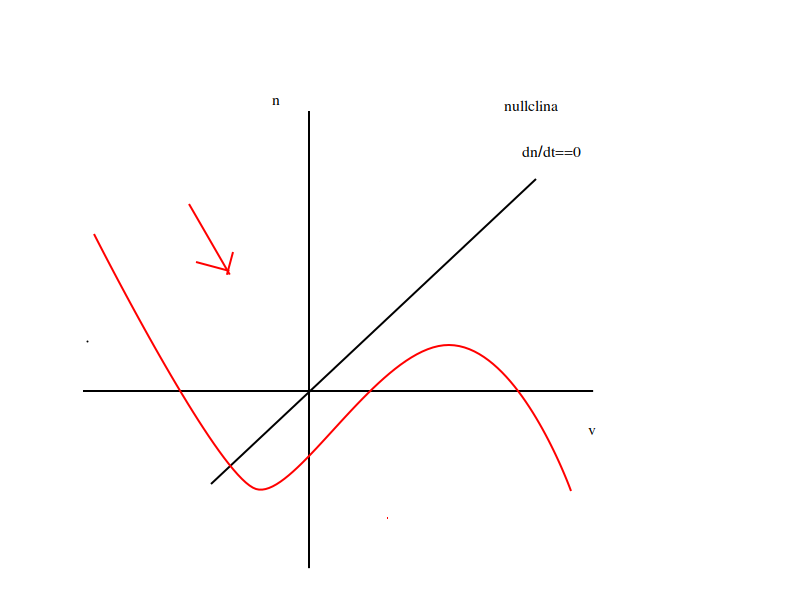
\includegraphics[width=0.45\textwidth]{1.png}
\end{figure}
Estas curvas cumplen por ejemplo

\begin{equation}
	dn/dt ==0 
\end{equation}

Los puntos fijos son las intersecciones de las nullclinas, donde la variacion de ambas es nula. En cada región de las nullclinas, pueden tener regiones que tiene ``flechas'' que se cierran, eso no implica que es oscilatorio o estable. Para saber eso necesitamos estudiar la estabilidad de un sistema de 2x2. 

\subsection{estabilidad de un sistema de 2x2}

Tengo el punto fijo por la intersección $(v_0,n_0)$ ¿como  hago el calculo de estabilidad? Armo la matriz, Para eso uso las ecuaciones, derivo y las evalúo en el punto fijo
\[
\begin{matrix}
	f'(v_0) &  -1   \\
	\nicefrac{b}{tn}& \nicefrac{-a}{tn} \\
\end{matrix}
\]

Podemos armar el polinomio característico, como una matriz de 2x2, hallar las soluciones es fácil

\begin{equation}
	\lambda = T \pm \sqrt{T^2 - 4D}/ 2
\end{equation}

donde T es la traza y D es el determinante.

\begin{figure}[htbp]
	\centering
	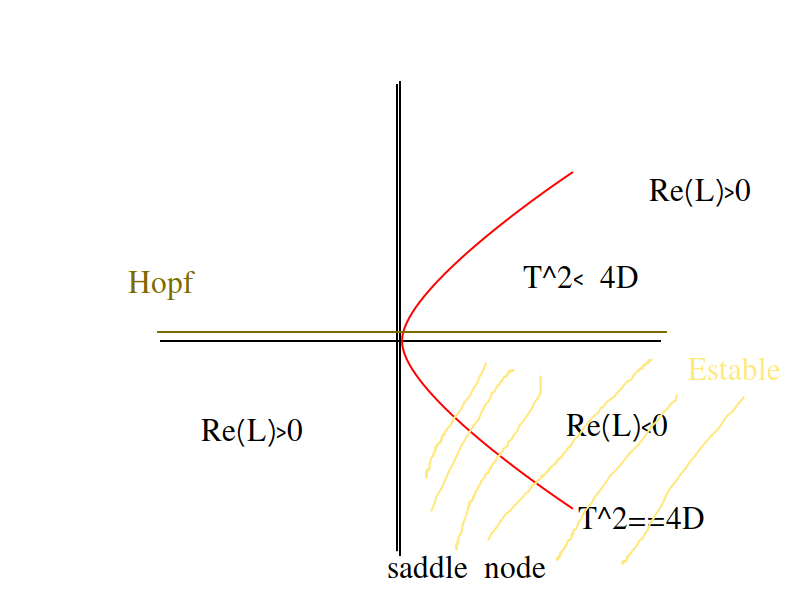
\includegraphics[width=0.45\textwidth]{2.png}
\end{figure}



Si estudio como varían las raíces del polinomios, donde se hacen negativos, positivos para la parte real e imaginaria, puede tener distintas zonas. Estas características depende del valor de f'(V0) por ejemplo si es positivo es inestable, y si el negativo estable. La frecuencia con la que gira si es estable es la parte imaginaria de los auto-valores.

\begin{figure}[htbp]
	\centering
	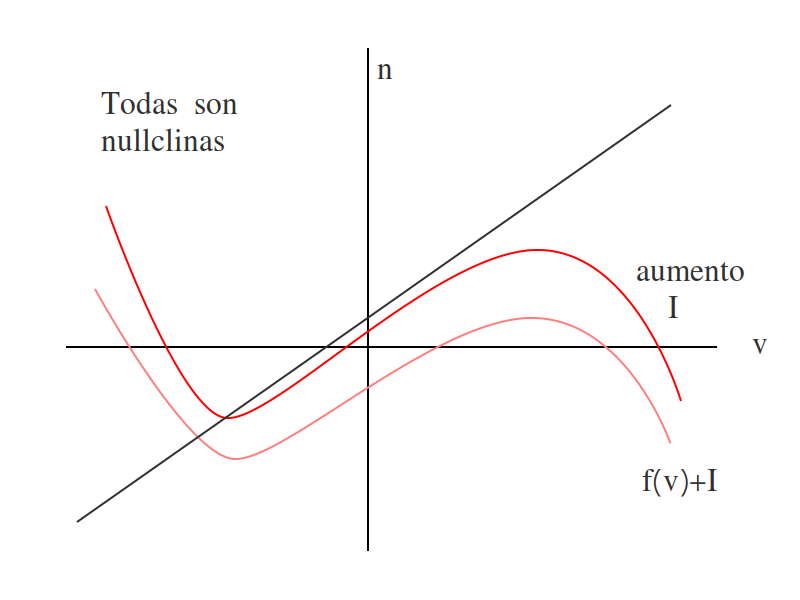
\includegraphics[width=0.45\textwidth]{3.png}
\end{figure}



Puedo ir corriendo la curva hasta llegar el punto que el mínimo de la cubica coincide con la recta. Incluso hasta cambiar el signo de los valores de las raíces, cambiando de inestable a Hopf. En este modelo no hay saddle node.

\subsection{Rebote post-inhibidor}

\begin{figure}[htbp]
	\centering
	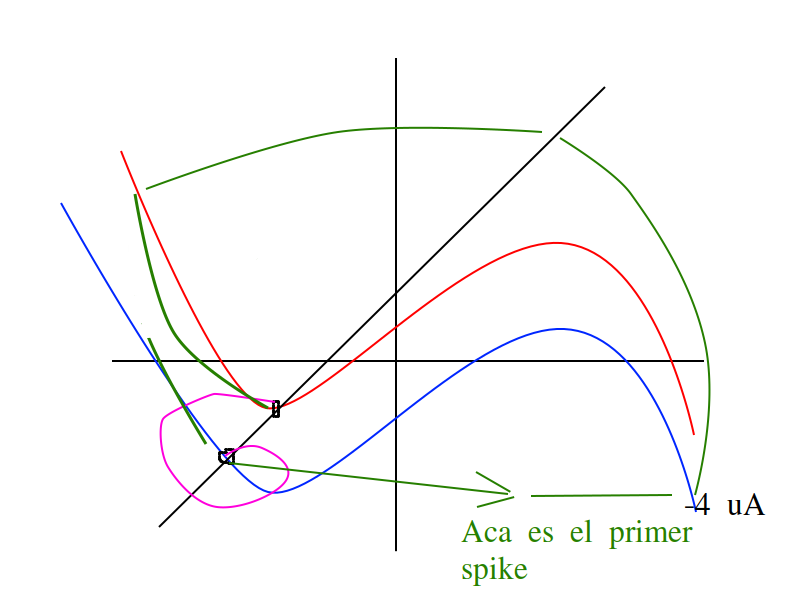
\includegraphics[width=0.45\textwidth]{4.png}
\end{figure}


Lo que pasa en el ejercicio cuando le pongo el -4, voy cambiando a los nuevos puntos fijos, así fue como va al ``nuevo'' equilibrio, en una sola vuelta. 


\subsubsection{Modelo de Morris-Lecar}
\begin{equation}
	\frac{dV}{dt} = f(V) -n + I
\end{equation}
N es la variable restitutiva, I la corriente.

\begin{equation}
	\tau_n \frac{dn}{dt}= -an + b*h(v)
\end{equation}

la h(v) puede ser un sigmoide por sigmoide por ejemplo

\begin{figure}[H]
	\centering
	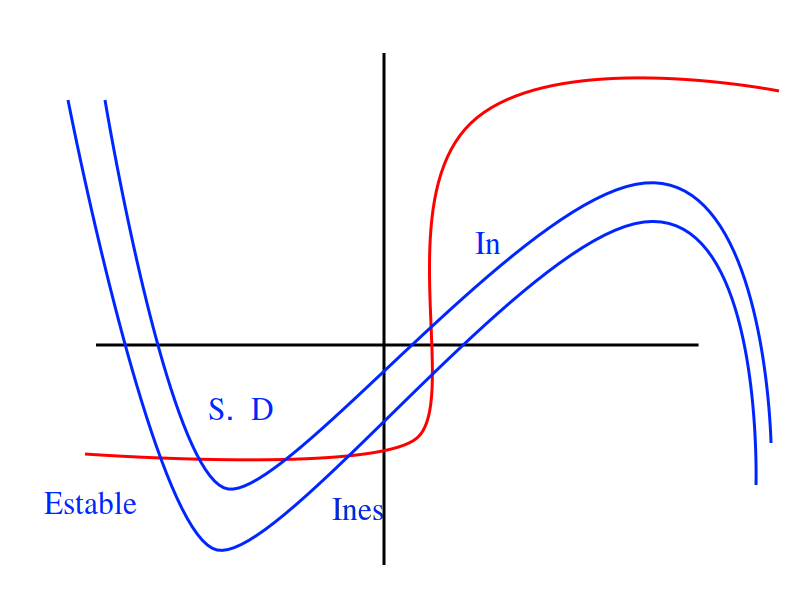
\includegraphics[width=0.45\textwidth]{5.png}
\end{figure}

COn la sigmoide puedo generar un saddle node, peude calcular el tiempo con la raiz de I, como la clase pasada. Con el sigmoide puedo tener muchos puntos de intersección.


\subsection{Interacciones neuronales}

Como las neuronas interactuan entre sí, mediante distintos mecanismos. Una por ejemplo es  la sinapsis químicas. 

\begin{figure}[htbp]
	\centering
	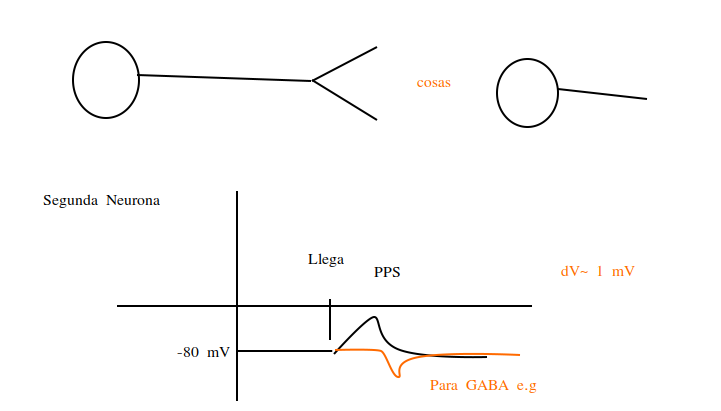
\includegraphics[width=0.5\textwidth]{+6.png}
\end{figure}

Como escribimos esto en ecuaciones? Agregamos a un término del tipo $-g_{syn}(t)(V-V_{syn})$.Este tiene un cuenta la curvita de cuando se abre al canal. (fig 6)

Otro forma que tienen de interactuan las neuronas son las sinapsis electrotónicas. Básicamente es un canal entre membranas que deja pasar iones, el término es $-g_{electrotonico}*(V-V')$

\section{Clase anterior falté.}

Deadline de la práctica 2: Marzo 11.

\section{28/02/2020}

Deadline de la práctica 3:

\subsection{Propiedades estadísticas de trenes de spikes}

Hasta ahora describimos a las neuronas individuales, modificando la corriente que entra, o cambiando sus propiedades. Al fin y al cabo, yo solo puedo acceder a ellas desde afuera, no puedo controlar la corriente en la práctica. Aunque de alguna manera  si podemos controlar el entorno donde está en un ser vivo, es decir, podemos estimular al ser de distintas maneras.

Dado un estimulo, el output no es determinista. En la realidad no controlamos todas la entradas: esto es la variabilidad entre trials. Tenemos los spikes, puedo calcular el histograma de ISI (inter spike interval), para saber la media $<ISI>$ o $<ISI^2>$. También la variancia $\sigma^2$, y con ella podemos calcular un coeficiente de variabilidad $CV = \nicefrac{\sigma_{ISI}}{<ISI>}$.

\begin{figure}[H]
	\centering
	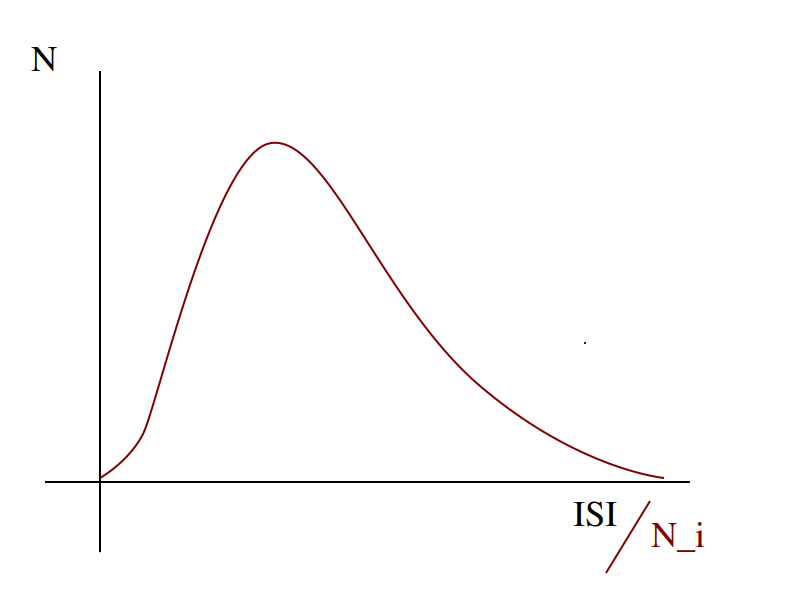
\includegraphics[width=0.45\textwidth]{2-1.png}
	\caption{Distribución de intervalos de tiempo entre spikes o número de spikes, no necesariamente son iguales.}
\end{figure}

Cuando realizo un trail, puedo obtener $N_i$ spikes, y también puedo hacer el mismo análisis que el $<ISI>$, es decir, $<N_i>$ etc, excepto que ahora se ahora el factor de Fano: $F = \nicefrac{\sigma^2}{<N>}$.


{\bf Proceso de Poisson}: consideramos que los potenciales de acción son independientes entre sí. Tomando un $dt$, $\nicefrac{dP_{spike}(A)}{dt} = F$, en cambio para que no haya spikes, $P_{no spike}(A \rightarrow A+dt) = 1 -F dt$. 
Supongamos que tenemos este proceso, ¿Cual es $P_{ISI}$? Dado un intervalo de tiempo n*dt, $P_{ISI}dt=(1-fdt)^{n-1}fdt \approx e^{-fdtn}fdt = e^{-f\,ISIS}fdt$, entonces, como la pdf ya está normalizada, lo interesante es 

\begin{equation}
	\int P_{ISI} ISI dt = 1/f = <ISI>
\end{equation}

Donde f es la frecuencia media entre spikes.  Ahora si calculamos $<ISI^2>$, por cosas que no quiero escribir y una $\Gamma(3)$, sale que $<ISI^2>= 2/f^2$. Donde entonces $\sigma= 1/f$, por lo que $CV=1$, este valor es una característica de Poisson.


Ahora para calcular el factor de Fano, no depende  del ISI porque son definiciones independientes. Para calcular el $P(N)$, tenemos N spikes en un intervalo de tiempo T, tomamos un dt pequeño y escribimos

\begin{equation}
	P(N) = \frac{(fdt)^N (1 - fdt)^{T/dt - N}x (T/dt)!}{N!(T/dt-N)!}
\end{equation}

Ahora si $N<<T/dt$

\begin{equation}
		P(N) = (fdt)^N e^{-fT} (T/dt)^N= (fT)^N e^{-fT}/N!
\end{equation}

Lo lindo de esta ecuación es que ya está normalizada, además $<N> = fT$, entonces $\sigma^2=<N>$, entonces $F=1$.


{\bf Renewal process:} es cuando $CV=F^2$. Son procesos donde el  spike solo depende del spike anterior.


\subsection{Integrador}

Es como  un Integrate-and-Fire, pero la resistencia es infinita. Entonces ahora tenemos,

\begin{equation}
	\nicefrac{dV}{dt}= I,
\end{equation}
donde si proponemos $I=\sum \alpha \delta(t-t_i)$, si soluciono el problema, tengo un escalón. Supongo que necesito llegar a un $V_th$ para generar un spike. 

\begin{figure}[H]
	\centering
	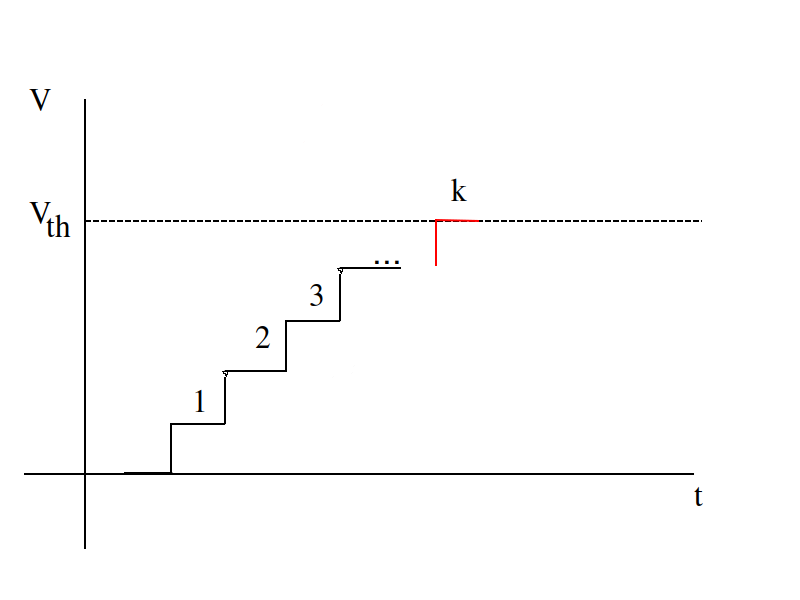
\includegraphics[width=0.45\textwidth]{2-2.png}
	\caption{A cada spike aumenta la tensión en $\alpha$}
\end{figure}

Sabemos que necesitamos $k=V_{th}/\alpha$ spikes para alcanzar el $V_{th}$. Para dado un tiempo T, ¿cual es la probabilidad de haber tenido k-1 spikes antes del K en T?

\begin{equation}
	P(T)=\frac{(fT)^{k-1} e^{-fT}f}{(k-1)!}
\end{equation}

Esta distribución es llamada $\Gamma_k(T)\approx (fT)^{k-1}e^{-ft}$ , si k es muy grande, la  distribución es muy picuda, en cambio si k es chico, es básicamente es una exponencial.


Ahora si tengo que los spikes van separandose en el tiempo, puede ser que la estimulación va bajando en frecuencia. Definimos $CV2= \frac{<|ISI_{n+1}-ISI_N|>}{2<|ISI_{n+1}+ISI_N|>}$. Si es poisson $CV2=CV$


{\bf Esto lo vamos a hacer en la práctica}

Para calcular la tasa de disparo efectiva, o  tasa de disparo subyacente, tengo que usar cada experimento, elegir un intervalo de tiempo y cuento cuantos spikes hubieron en total en ese intervalo en todos los experimentos.

\begin{figure}[H]
	\centering
	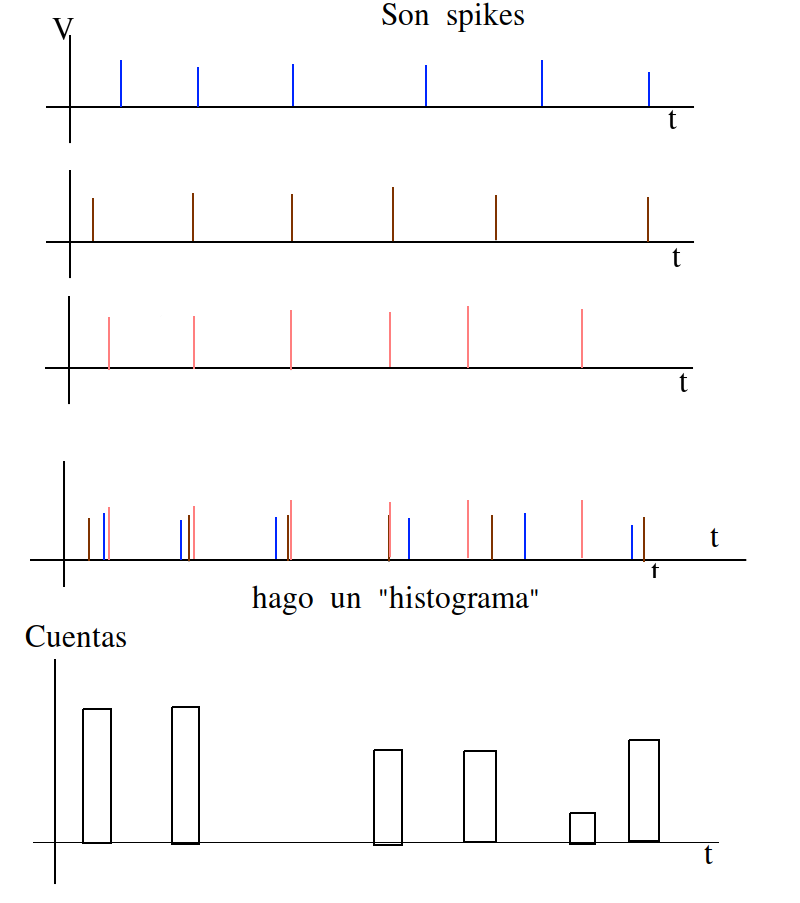
\includegraphics[width=0.45\textwidth]{2-3.png}
	\caption{A cada spike aumenta la tensión en $\alpha$}
\end{figure}

Para la practica 3: 
\begin{itemize}
	\item Calcular CV,F
	\item si es renewal o no
	\item la r(t) (tasa subyacente)
\end{itemize}


\section{04/03/2020}

\subsection{¿Cómo estimar el estimulo desde la respuesta?}

Consideremos las funciones de $s(t)$ y $r(t)$ para estimulo y respuesta efectivamente. 

\begin{figure}[H]
	\centering
	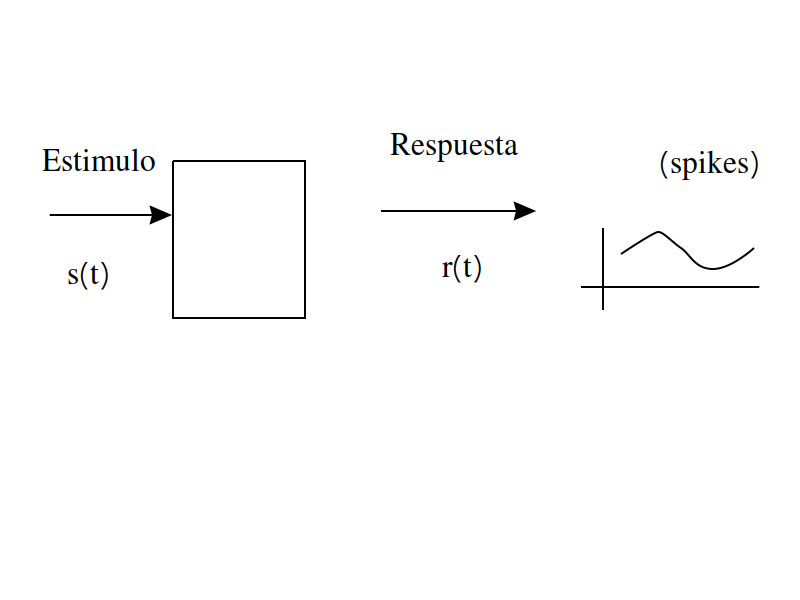
\includegraphics[width=0.45\textwidth]{3-1.png}
	\caption{La cajita es el cerebro}
\end{figure}

Sabemos que dado la red, la respuesta depende del estímulo, por que podemos escribir la relación $r(t) =  F[s(t')]$ con $t<t'$ para respetar causalidad. La funcional puede expandirse en series de Volterra, un ejemplo es lo siguiente:

\begin{equation}
	r(t) = F[s(t')]= r_0 + \int_0^\infty d\tau D(\tau) s(t-\tau) + \int_0^\infty d_{\tau_1} d \tau_2 D(\tau_1, \tau_2) s(t-\tau_1) s(t-\tau_2)
\end{equation}
donde $D(\tau)$ es conocida para el kernel lineal (o Wiener) y $r_0$ es una constante.

Proponemos un kernel y obtenemos una función $r_{est}(t)$, y lo que voy a buscar es minimizar la función error $E = \int_o^T dt (r_{est}(t)-r(t))$, por que buscamos que $\nicefrac{dF}{dr_0}=0$ y $\nicefrac{dE}{dD}$.

Estas son derivadas funciones, para hacer numéricamente esta cuenta, se hace así.

\begin{itemize}
	\item El argumento t->$i\Delta$ y $\tau \rightarrow j\Delta$
	\item Dividimos el rango $0-T$ en $\Delta$, donde $T= N \Delta$
	\item 
	\begin{equation}
		E= \Delta \sum_{i=0}^{T/\Delta} (r_{est}(i\Delta) - r(i\Delta))^2
	\end{equation} 

	\item ahora la función 
	\begin{equation}
	r_{est}(i\Delta) = r_0 + \Delta \sum^\infty_{j=0} D(j\Delta)s(i\Delta - j\Delta)	
	\end{equation}
	\item Reescribimos
	\begin{equation}
		r^{est}_i = r_0 + \Delta \sum^\infty_{j=0} D_j s(i\Delta - j\Delta)	
	\end{equation}

	\item Se busca minimizar $\nicefrac{dF}{dr_0}=0$ y $\nicefrac{dE}{dD}$, que se transforman en la discretización como $\nicefrac{dE}{dr_0}=0$ y $\nicefrac{dE}{dD_j}$.
	\item 
	\begin{equation}
		\frac{dE}{d D_k} = 0 = 2\Delta \sum_{i=0}^{T/\Delta} (r^e_i - r_i)\frac{dr^E_i}{d D_k}
	\end{equation}
	\begin{equation}
		\frac{dr^E_i}{d D_k}= \Delta S_{i-k}
	\end{equation}

	\item Finalmente nos quedan las siguientes ecuaciones para las funcionales

	\begin{equation}
		\sum_{i=0}^{T/\Delta}= (r_i - r_0)s_{i-k} = \Delta \sum_j D_j \big[ \sum_i s_{i-j} s_{i-k}\big]
	\end{equation}
	\item Con esta expresión puedo llevar al continuo tomando $\Delta \rightarrow 0 $
	\item Aun nos falta el término $\nicefrac{dE}{dr_0}$. Para esto vamos a tomar la expresión que habíamos obtenido para $r_0$
	\begin{equation}
		\frac{dE}{dr_0} = 0 = 2 \sum [r_0 + \Delta \sum D_j s_{i-j} -r_i]
	\end{equation}

	Porque esto es igual  a 0, tenemos que

	\begin{equation}
		\int_0^T dt [r_0 +  \int d\tau \sum [r_0 + \Delta \sum D_j s_{i-j} -r_i]D(\tau) s(t-\tau) -r(t)] =0
	\end{equation}
	Por lo tanto

	\begin{equation}
		r_0 = \frac{1}{T} \int r(t)dt - \frac{1}{T} \int d\tau dt D(\tau) s(t-\tau)
	\end{equation}
	\begin{equation}
		r_0 = <r(t)> - \int d\tau D(\tau)<s(t-\tau)>
	\end{equation}
	\item Definimos la función de correlación entre estimulo-respuesta como
	\begin{equation}
		Q_{r,s} (0, \tau') = \int d\tau D(\tau') Q_{s,s}(\tau, \tau')
	\end{equation}
	\begin{equation}
			Q_{r,s} (-\tau') = \int_{-\infty}^{\infty} d\tau' D(\tau') Q_{s,s}(\tau- \tau')
	\end{equation}
	Donde $Q_{s,s'}$ es la función de correlación entre estimulos
	\begin{equation}
		Q_{s,s} (\tau, \tau') = \int dt s(t-\tau)s(t-\tau') \rightarrow Q_{s,s}(\tau, \tau')
	\end{equation}

	\item Haciendo la transformada de Fourier (hay muchos pasos que no escribi porque no) 
	\item 
	\begin{equation}
		D(\tau) = \frac{1}{2\pi} \int^{\infty}_{\infty} d\omega \frac{Q_{r,s}(-\omega)}{Q_{s,s}(\omega)} e^{-iw\tau}
	\end{equation}

\end{itemize}


Propongamos ahora que el estimulo es ruido blanco, esto tiene la característica que la correlación entre dos tiempos distintos en nula: $Q_{s,s}(\tau - \tau') =  \sigma^2 \delta(\tau-\tau')$. Por lo que, la ecuación anterior conlleva que $D(\tau) = \frac{Q_{rs}(-\tau)}{\sigma^2}$

¿Que pasa si las respuestas son spikes?  

Para la práctica 3:

\begin{itemize}
	\item Asumimos que el estimulo es ruido blanco 
	\item $Q_{r,s}(-\tau) = \sum_{spikes} S(t_{spike} - \tau)$
	\item $D(\tau)= \nicefrac{Q_{rs}}{\sigma^2}$ 
\end{itemize}



\section{06/03/2020}

\subsection{Redes neuronales artificiales}

{\sl Sistemas neuronales como un sistema biologico, desde distintos puntos de vista. Ahora ¿de lo anterior podemos aplicar? ¿Cuales son los conceptos principales? Una neurona es algo que recibo un input y da un output. El output puede depender de un threshold. 
}
\begin{itemize}
	\item Las neuronas son elementos simples que transforman una entrada a una salida dado un umbral.
	\item Las neuronas están conectadas entre sí, a esto se lo denomina {\sl arquitectura}.
	\item La función que realizan los sistemas neuronalespuede ser aprendida mediante ejemplos: aprendizaje a partir de ejemplos.
	\item Los sistemas son altamente redundantes. Ejemplo: Parkinson, los síntomas empiezan cuando se destruye casi el 80\% de las neuronas, debido a la redundancia.
	\item Tip: Simplificar como funciona la neurona.
	\item ¿Cómo? Si $in>umbral \rightarrow out$
	\item Entrada $h_i(t)$ y salida $n_i(t)={0,1}$
	\item $n_i(t) = \Theta(h_i(t) - T)$, donde T es el umbral.
	\item Suponiendo que la entrada depende de la salida de otras neuronas, $h_i(t) = \sum_j w_{ij}n_i(t)$, donde $w$ puede ser negativo!
	\item La salida puede ser continua, donde $f_i$ varía entre $0-\infty$. La relación entre la entrada $f_i(t) = F(h_i(t)-T)$.
	\item La topología (como está armada la red) está en la matriz $w_{ij}$. Pueden ser entradas nulas, negativas. Me dice que está conectado con que
\end{itemize}

En la materia vamos a estudiar dos arquitecturas principales:

\begin{enumerate}
	\item {\bf Arquitectura Feed-Forward o Multicapa}

Las neuronas están organizadas en capas. Un neurona sólo pueden mandar señales a la siguientes capas, la señal no puede volver a capas anteriores. ¿Por qué sirve? Porque cuando una neurona llega a un valor, no puede cambiar debido a las neuronas siguientes. implementa un mapeo entrada-salida.

	\item {\bf Redes totalmente conexas}

Bueh, es lo opuesto. Es altamente no trivial: tras la condición inicial el sistema evoluciona, puede converger a un punto fijo o un equilibrio dinámico. Puedo pensar al punto fijo como una memoria que almacené de alguna forma: modelo de memoria, generar patrones cíclicos. La implementación de la condición inicial involucra a todas las neuronas.

Si la matriz $w_{ij}$ es simétrica, el sistema converge a un punto fijo siempre. 


\end{enumerate}


\begin{itemize}
	\item {\sl ¿Qué funciones podemos implementar con una red multicapa?}
	\begin{itemize}
		\item Regresión
		\item Clasificación
		\item Segmentación
		\item Descubrir cuales son las dimensiones relevantes, dado un set de datos
	\end{itemize}
	\item {\sl ¿Cuántas entradas puede tener la red} Problema de Capacidad: Cual es problema más grande que puede resolver mi red, o cual es la mínima red que resulva un problema. La medida de cuan grande es la red de neuronas es por la cantidad de neuronas y conexiones.
	\item {\sl ¿Cómo se encuentra la red que soluciona un problema?}
	\begin{itemize}
		\item ¿Cómo encuentro los parámetros que necesito para resolverla? Problema de aprendizaje. Yo quiero que este problema se resuelva mediante ejemplos. Luego de esto.
		\item ¿Como se si puede resolver un nuevo set si me red ya aprendió? Problema de generalización. 
		\item Transferencia: cual es la capacidad de dar el resultado correcto con una red de datos nueva/ nueva estadística.
	\end{itemize}
	\item {\sl ¿Se puede aprender sin supervisión?} Yo quiero que la relación in/out tenga un valor.
\end{itemize}

\subsubsection{Feed-Forward}
La más fácil es un sola neurona LOL. La salidad $O$ está dada por $O= g(h)$, donde la función g puede ser lineal o heaviside u otra función, y el valor de $h= \sum_j^N w_j x_j$,  donde $w$ es el peso y $x$ es la entrada. Muchas veces se escribe $g(h-T)$, pero puedo implementar de otras formas. Una red, con suficientes capas y conexiones, es capaz de aproximar cualquier?? función no lineal  arbitraria.

El caso más simple es que $g$ tenga como salida dos valores: $\{ 0, 1\}$. A esto se le llama el {\sl perceptron}: es un clasificador binario.

Fig 4-1

Con un perceptron puedo clasificar en si o no, básicamente lo que hace  la red es poner un hiperplano que separe de $h=0$. Este problema es linealmente separable. Esto es una sola capa. Si un problema es linealmente separable: sé que la solución va a converger en un tiempo finito con un perceptron.

Fig 4-2

En este caso el perceptron no puede solucionar. No es linealmente separable. 


\subsubsection{Algoritmo del perceptron}

El vector de datos $x_j^{\mu}$ con $\mu$:1,..,$\rho$ (que vector estoy trabajando, índice de la base de datos y en la neurona j) donde $\rightarrow z^\mu=\pm1$ son las salidas que yo quiero.

\begin{itemize}
	\item Elijo conexiones iniciales $w_j$ aleatorias y pequeños
	\item Elijo un $\mu$
	\item Calculo $sgn\big(\sum^N_{j=1} w_j x_j^\mu \big) = O^{\mu}$
	\item Para calcular que variación debo hacer para cambiar los pesos. Donde $\eta$ y $\kappa$ es el famoso hiperparámetro.
	\begin{equation}
		\Delta w_j = \eta \Theta(N\kappa - h^\mu z^\mu) z^\mu x_j^\mu 
	\end{equation}
	¿Qué significa el $\Theta$? Donde es N es número de elementos/neuronas, y el $N\kappa$ es el factor de seguridad
	\item[x] Y se repite, yo elijo como se va a elegir el nuevo j.
\end{itemize}

{\bf Convergencia del algoritmo: Teorema de Convergencia}

Existe una solución tal que $sgn(\sum_j w_jx_j^\mu)=z^{\mu}= \pm 1$ que puedo escribir como $sgn(\sum_j w_jx_j^\mu z^\mu)=1$ por lo tanto $\vec w \vec x^\mu z^\mu > 0$ para todo $\mu$. Defino una distancia 
\begin{equation}
	D(\vec w) = \frac{min_\mu(\vec w . \vec x^\mu \, z^\mu)}{|\vec w|}
\end{equation}

Hay una solución óptima $\vec w ^{opt}$ que maximiza D($\vec w$)

Después de aplicar el algoritmo M veces, llego a una relación del tipo:

\begin{equation}
	M \le \frac{N(\eta + 2\kappa)}{\eta D^2(\vec w ^{opt})}
\end{equation}

(está en el herzt)

\section{11/03/2020}

\subsection{Continuación del perceptron: problema de capacidad}

¿Hasta que punto un problema es linealmente separable? Tengo $p$ vectores de entrada, con $n$ dimensiones. 

\begin{figure}[H]
	\centering
	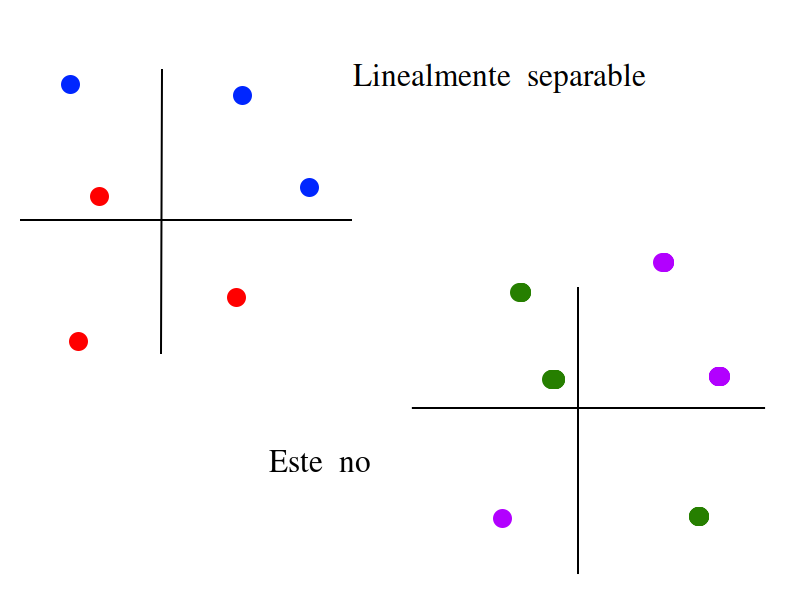
\includegraphics[width=0.5\textwidth]{5-1.png}
\end{figure}
Considerando la figura anterior, ¿cuantas formas de colorear, dado dos colores, esa misma cantidad de datos? El color es la clasificación (si, no). 

En total, tenemos $2^P$ es el número de problemas posibles. Para los problemas linealmente separables, eventualmente los datos pueden repetirse en alguna de las n-componentes, por lo tanto los problemas linealmente separables, $C(p,n)$.

\begin{figure}[htbp]
	\centering
	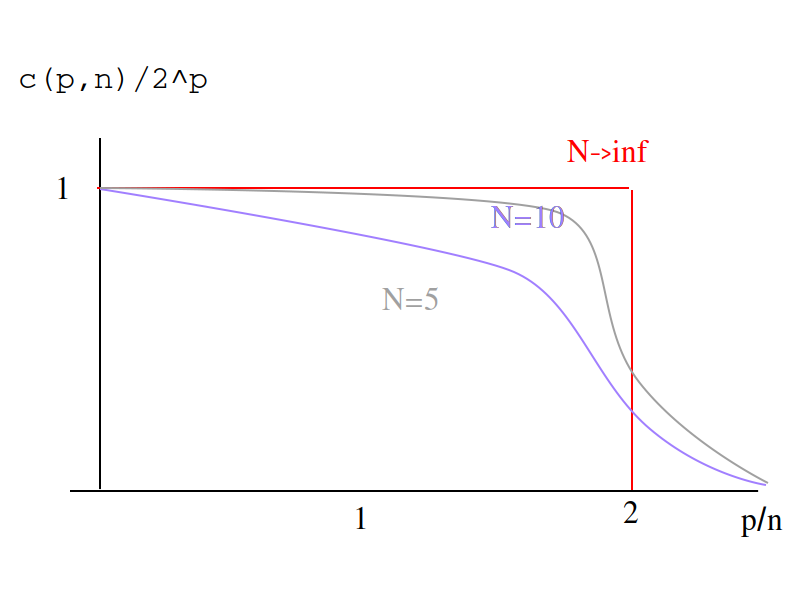
\includegraphics[width=0.5\textwidth]{5-2.png}
\end{figure}

Cuando la dimensión es muy grande, la curva tienden a un escalón, por lo que tenemos un límite para $p$, $p_{max}= 2n$ para $n>>1$.

Para demostrar eso, consideramos $c(1,n)=2$ porque puedo colorear de dos formas distintas, análogamente $c(p,1)=2$. Ahora, ¿cuánto vale $c(p+1,n)$ si ya conozco el valor de $c(p,n)$? 

\begin{figure}[H]
	\centering
	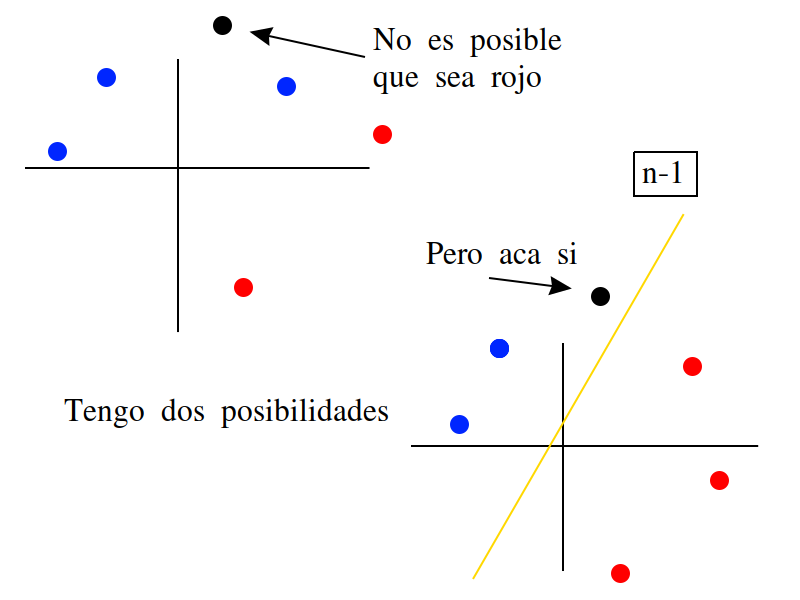
\includegraphics[width=0.5\textwidth]{5-3.png}
\end{figure}

Dependiendo de donde caiga el nuevo punto, puede ser posible o no que tenga alguno  de los dos colores. Hay condiciones donde no, otras que sí. Cuando es posible que tenga los dos colores, lo que se hace es considerar el hiperplano de dimensión de n-1 que pasa por ese punto, ahora tengo otro nuevo problema donde tengo que ordenar los p vectores en este. Por lo tanto. $c(p+1, n) = c(p,n) + c(p, n-1)$, donde el primer término es cuando no tiene que ver los casos donde no tiene opción, y el segundo es por el hiperplano.


Tenemos la relación de recurrencia y los casos base, y llegamos a que 
\begin{align}
	c(p,n)=&\binom{p-1}{0}c(1,n) + \binom{p-1}{1}c(1,n-1)\\
	&\dots + \binom{p-1}{p-1}c(1,n-p+1)\\
	&\text{Si } p \le n  \rightarrow c(p,n)=2^p 
\end{align}

Ahora si $p>n$
\begin{align}
	&c(p,n)=\binom{p-1}{0}c(1,n) + \binom{p-1}{1}c(1,n-1) \\
	&\dots + \binom{p-1}{n-1}c(1,1)\\
	&c(p,n)=2\times(\binom{p-1}{0} + \binom{p-1}{1}\dots + \binom{p-1}{n-1})\\
	&\text{Si }p=2n \rightarrow c(2n,n) = 2^{p-1}
\end{align}

Al final, lo que no vamos a ver, es que para el caso general, 
\begin{equation}
	c(p,n) = 2^{p-1} \bigg[ 1- erf \bigg( \sqrt{\frac{p}{2}} \big(\frac{2n}{p}-1\big)\bigg) \bigg]
\end{equation}

La gracia de todos esto, es que justamente, acá se ve que aumentando la dimensión, es decir agregando capas, puedo tener un problema linealmente separable. 

\subsection{Problema lineal}

Dada una entrada $\vec x ^\mu$, hago la cuenta y tengo un output $o ^\mu = \sum^N _j w_j x^\mu _j$, pero la salida deseada es $\sigma^\mu$. ¿Cómo soluciono los pesos si estas matrices no son cuadradas?

\begin{align}
	w_{j} = \frac{1}{N}\sum^P _{\mu,\nu=1} \sigma ^\mu (Q^{-1})_{\mu,\nu} x^\nu_j\\
	Q_{\mu,\nu}= \frac{1}{N} \sum^N_j x^\mu_j x^\nu_j
\end{align}
Como Q tiene una inversa si $x_i$ y $x_j$ son linelmente independientes, eso implica que en un sistema lineal, la capacidad es máxima cuando $P_{max}=N$

\dots

Para resolver en general usamos cuadrados mínimos. Definimos la función error $E(\{ w_j\}) = \nicefrac{1}{2} \big( \sigma^\mu - \sum w_j x_k^\mu \big)^2$. Ahora minimizando con un   $w_j$,
\begin{align}
	-\eta \frac{\partial W}{\partial w_j} = \Delta w_j \qquad \eta << 1
\end{align}
Haciendo la cuenta,  sale que
\begin{align}
    \Delta w_l &= -\eta \sum_\mu \bigg( \sigma ^ \mu - \sum_j w_jx_j^\mu\bigg) x^\mu_l\\
    \delta^\mu &= \sigma ^ \mu - \sum_j w_jx_j^\mu \quad \leftarrow \text{ADALINE}
\end{align}
%Otro problema surge cuando todos los puntos ya están alineados en un hiperplano. Bueno, ahora tenemos que considerar   

Considerando la clase anterior, cambiamos la función de Heaviside por la función $\delta ^\mu$.


\subsection{Problema no lineal continuo}

Considerando la función g continua y derivable, donde el output $o^\mu = g(\sum w_j x_j^\mu)$, definiendo la función de error (función de costo) como antes. Tenemos que

\begin{align}
    &\Delta w_l = -\eta \sum_\mu \bigg( \sigma ^ \mu - g(\sum_j w_jx_j^\mu)\bigg) x^\mu_l g'(\sum_j w_jx_j^\mu)\\
    &\text{Sea }h^\mu = \sum_j w_jx_j^\mu \\
    &\Delta w_l = -\eta \sum_\mu \bigg( \sigma ^ \mu - o^\mu\bigg) g'(h^\mu)  x^\mu_l\\
    &\text{Sea }\delta^\mu =  \bigg( \sigma ^ \mu - g(h^\mu)\bigg) g'(h^\mu)\\
    &\Delta w_l = -\eta \sum_\mu \delta^\mu  x^\mu_l\\
\end{align}

Por ejemplo, consideremos $g(h)=tanh(\beta h) \rightarrow g' = \beta (1-g^2)$, y me ahorro tiempo de cálculo.

Otra función de costo, es una basada en una especie de entropía, 

\begin{equation}
	E(\{ w_j \}) = \sum_\mu \bigg[  \frac{1+\sigma^\mu}{2} \log{\frac{1+\sigma^\mu}{1+o^\mu}} + \frac{1-\sigma^\mu}{2} \log{\frac{1-\sigma^\mu}{1-o^\mu}}  \bigg]
\end{equation}

Donde el peso es igual a 

\begin{align}
	\frac{\partial E}{\partial w_l} &=  \sum _\mu \bigg[  \frac{1+\sigma^\mu}{2} {\frac{-g'(h^\mu) x^\mu_l}{1+o^\mu}} + \frac{1-\sigma^\mu}{2} {\frac{g'(h^\mu) x^\mu_l}{1-o^\mu}}  \bigg]\\
	\frac{\partial E}{\partial w_l} &=  \frac{-g'(h^\mu) x^\mu_l}{2}\sum _\mu \bigg[  -\frac{1+\sigma^\mu}{1+o^\mu} + \frac{1-\sigma^\mu}{1-o^\mu} \bigg]\\
	&\text{Si g es tanh}\\
		\frac{\partial E}{\partial w_l} &= \sum_\mu \beta (o^\mu - \sigma^\mu) x_l^\mu
\end{align}


\begin{itemize}
	\item lineal
	\item no lineal
	\item algoritmo de aprendizaje que resuelve el problema
	\item Si pongo muchas capas lineales no gano nada
	\item pero si son no lineales
	\item boom Machine learning xdxdxdxdxd
\end{itemize}



\begin{itemize}
	\item Poner condiciones ininciales
	\item in and out
	\item error
	\item backpropagattion
	\item E vs t epoch para distintas $\eta$
	\item Interpretar los resultados como algo geometrico
	\begin{itemize}
		\item Como un sgn y no tanh
		\item la geometría 
	\end{itemize}
	\item Segundo ejer: xor en N puntos
	\item varias arquitecturas
	\item PAra el ejercicio 3
	\item generamos los ejemplos
	\item 
\end{itemize}

\end{document}